\begin{figure}[h]
  \center
  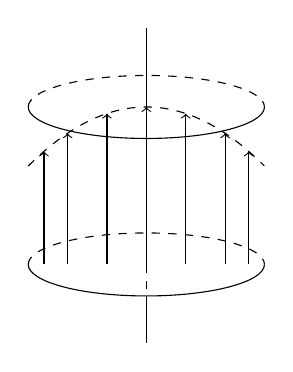
\begin{tikzpicture}
    % parametri
    \def \r{1.5}
    \def \h{2}
    \def \e{0.4}

    % ellissi
    % Armatura superiore
    \draw (-\r,\h) arc[start angle=180, end angle=360, x radius=\r, y radius=\e];
    \draw[dashed] (-\r,\h) arc[start angle=180, end angle=0, x radius=\r, y radius=\e];

    % Armatura inferiore
    \draw (-\r,0) arc[start angle=180, end angle=360, x radius=\r, y radius=\e];
    \draw[dashed] (-\r,0) arc[start angle=180, end angle=0, x radius=\r, y radius=\e];
    
    % Fili verticali
    \draw (0,\h) -- (0,\h+1);
    \draw [dashed] (0,0) -- (0,-\e);
    \draw (0,-\e) -- (0,-1);

    % profilo del campo
    \pgfmathsetmacro{\a}{\h/(2*\r*\r)}

    %\draw[domain=-\r:\r, samples=200, thick, black] plot (\x, {\h - \a*\x*\x});

    % funzione
    \def \f {\h - 3/4 * \a* \x *\x}
    \draw [domain = - \r : \r , samples = 200, dashed, black] plot (\x, {\f});
    
    % frecce campo elettrico
    \foreach \x in {-1.3 , -1, -0.5, 0, 0.5, 1, 1.3}{  \draw[->] (\x,0) -- (\x,{\f});}


  \end{tikzpicture}
  \caption{Profilo del campo elettrico nel condensatore}
  \label{figure: condensatore piano con profilo}
\end{figure}
